\chapter{音響エネルギ分布}
Strength$G$、話声に対応する明瞭度$D_{50}$、音楽に対応する明瞭度である初期/後期反射音エネルギ比$C_{80}$、初期残響時間$EDT$、初期側方反射エネルギ率$LF$、両耳間相互相関度$IACC$を算出した。
(A)矩形モデルにおける各種音響物理指標の解析結果を以下に示す。
\newpage
      \begin{minipage}{1\textwidth}
        \centering
          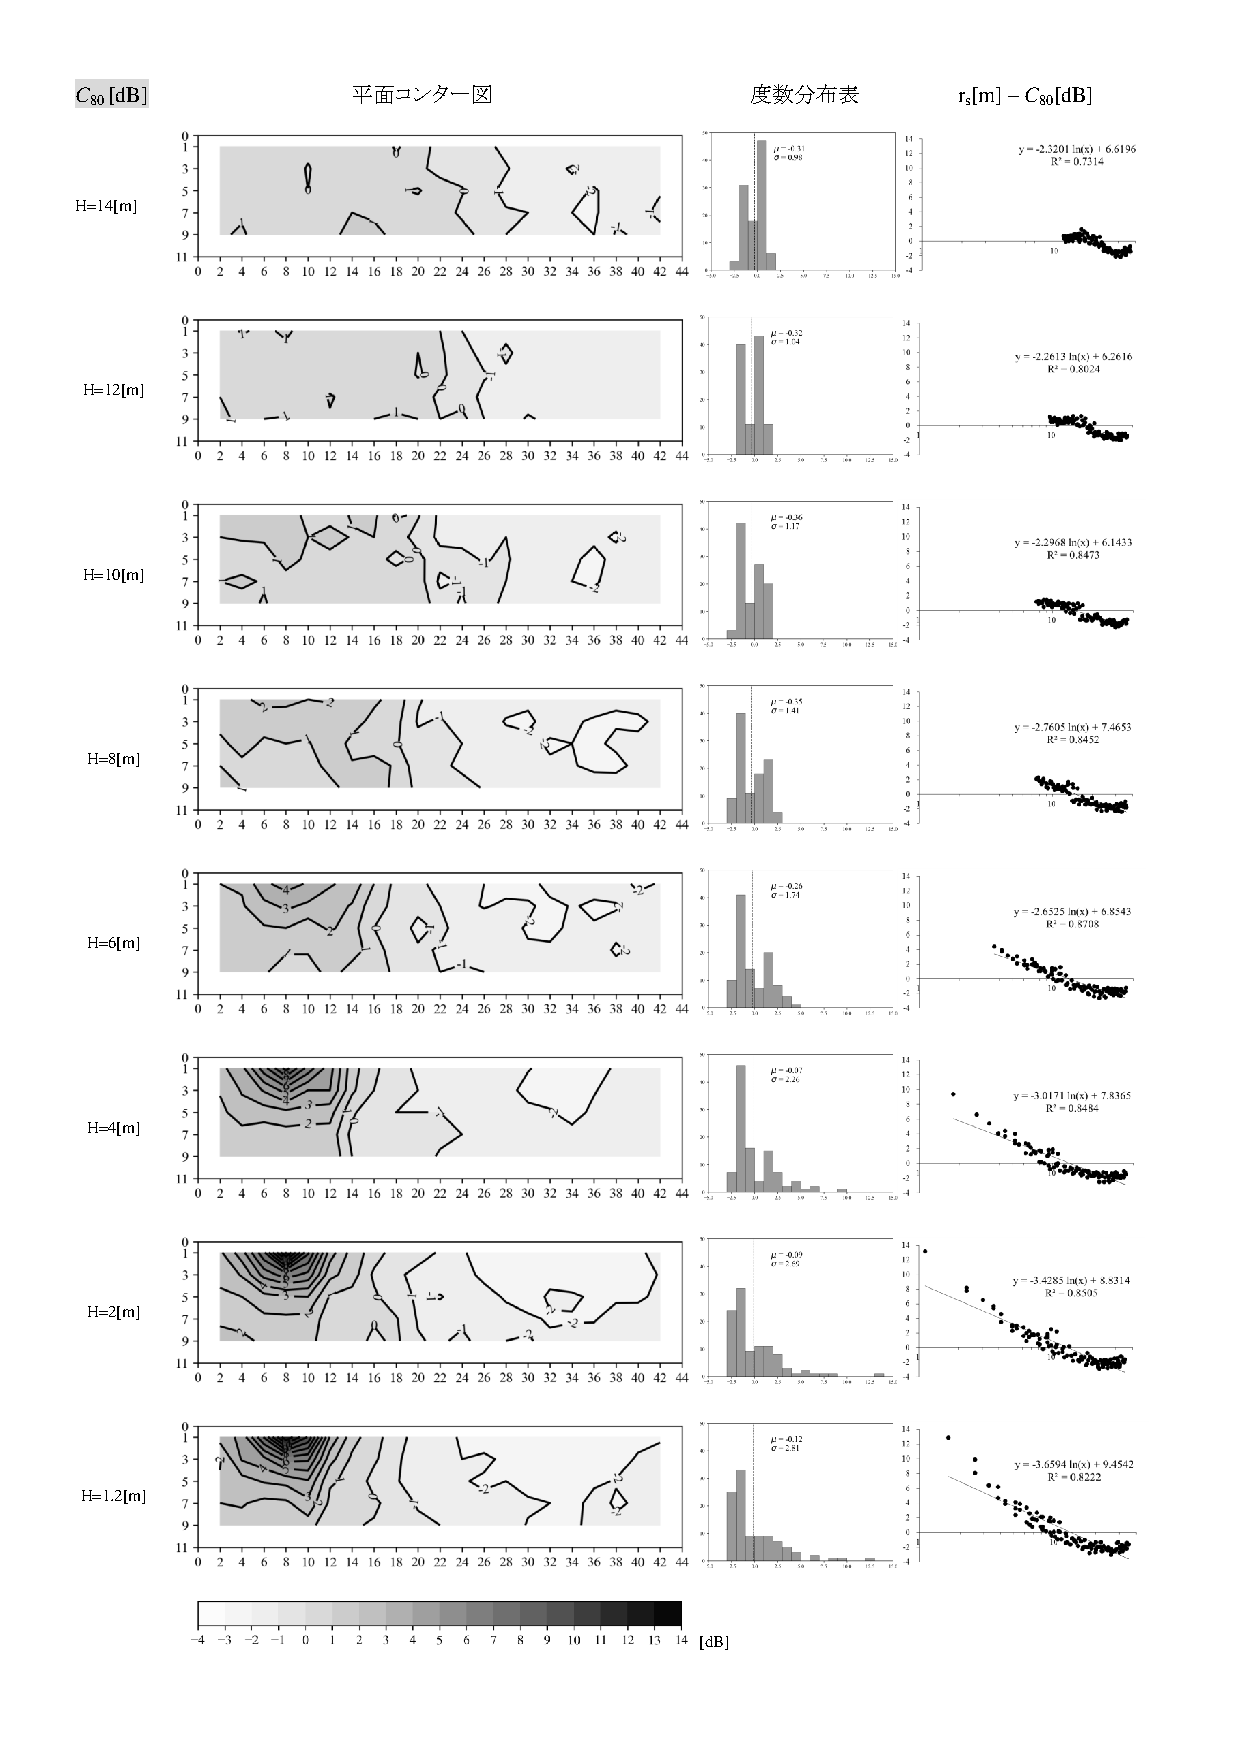
\includegraphics[keepaspectratio,width=1\hsize,angle=0]
                          {04_att/Onkyo_rec1.pdf}
      \end{minipage}
\newpage
      \begin{minipage}{1\textwidth}
        \centering
          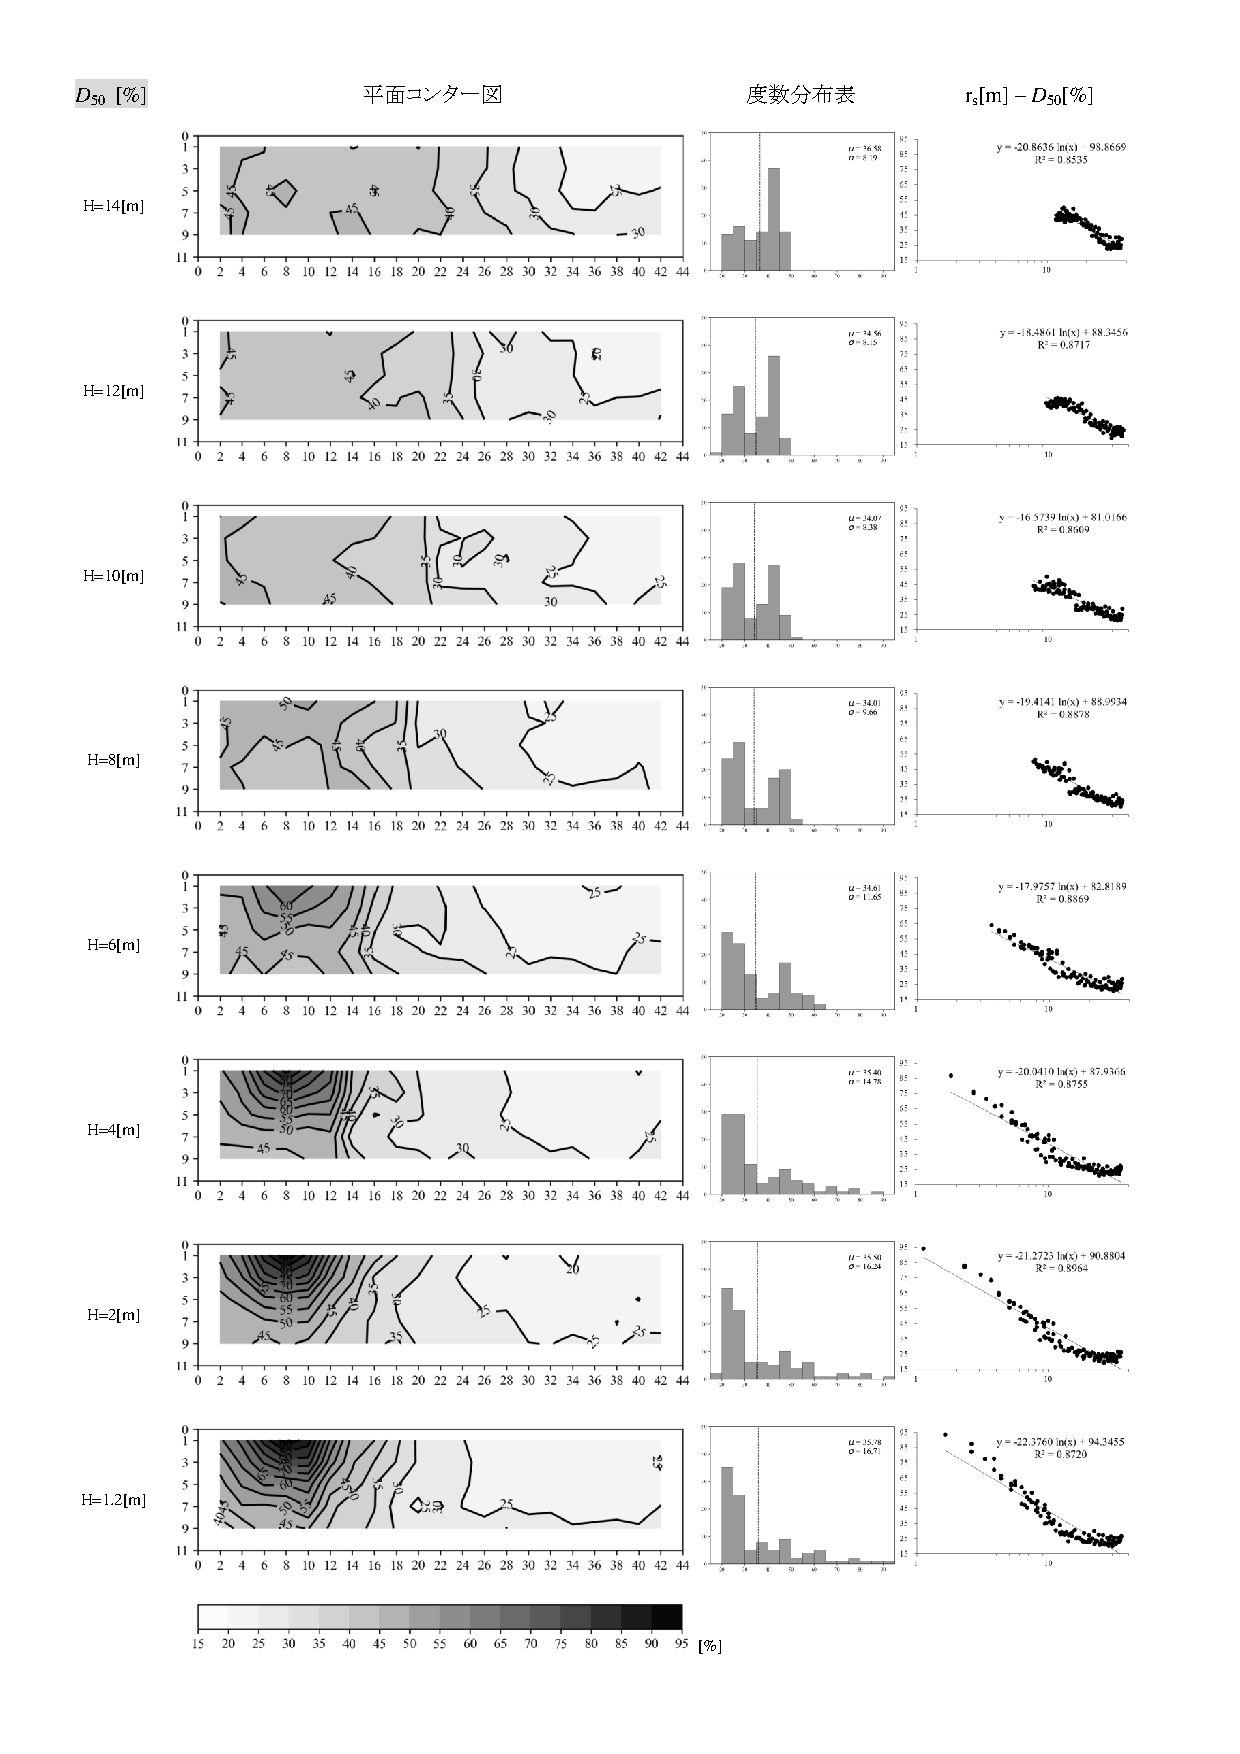
\includegraphics[keepaspectratio,width=1\hsize,angle=0]
                          {04_att/Onkyo_rec2.pdf}
      \end{minipage}
\newpage
      \begin{minipage}{1\hsize}
        \centering
          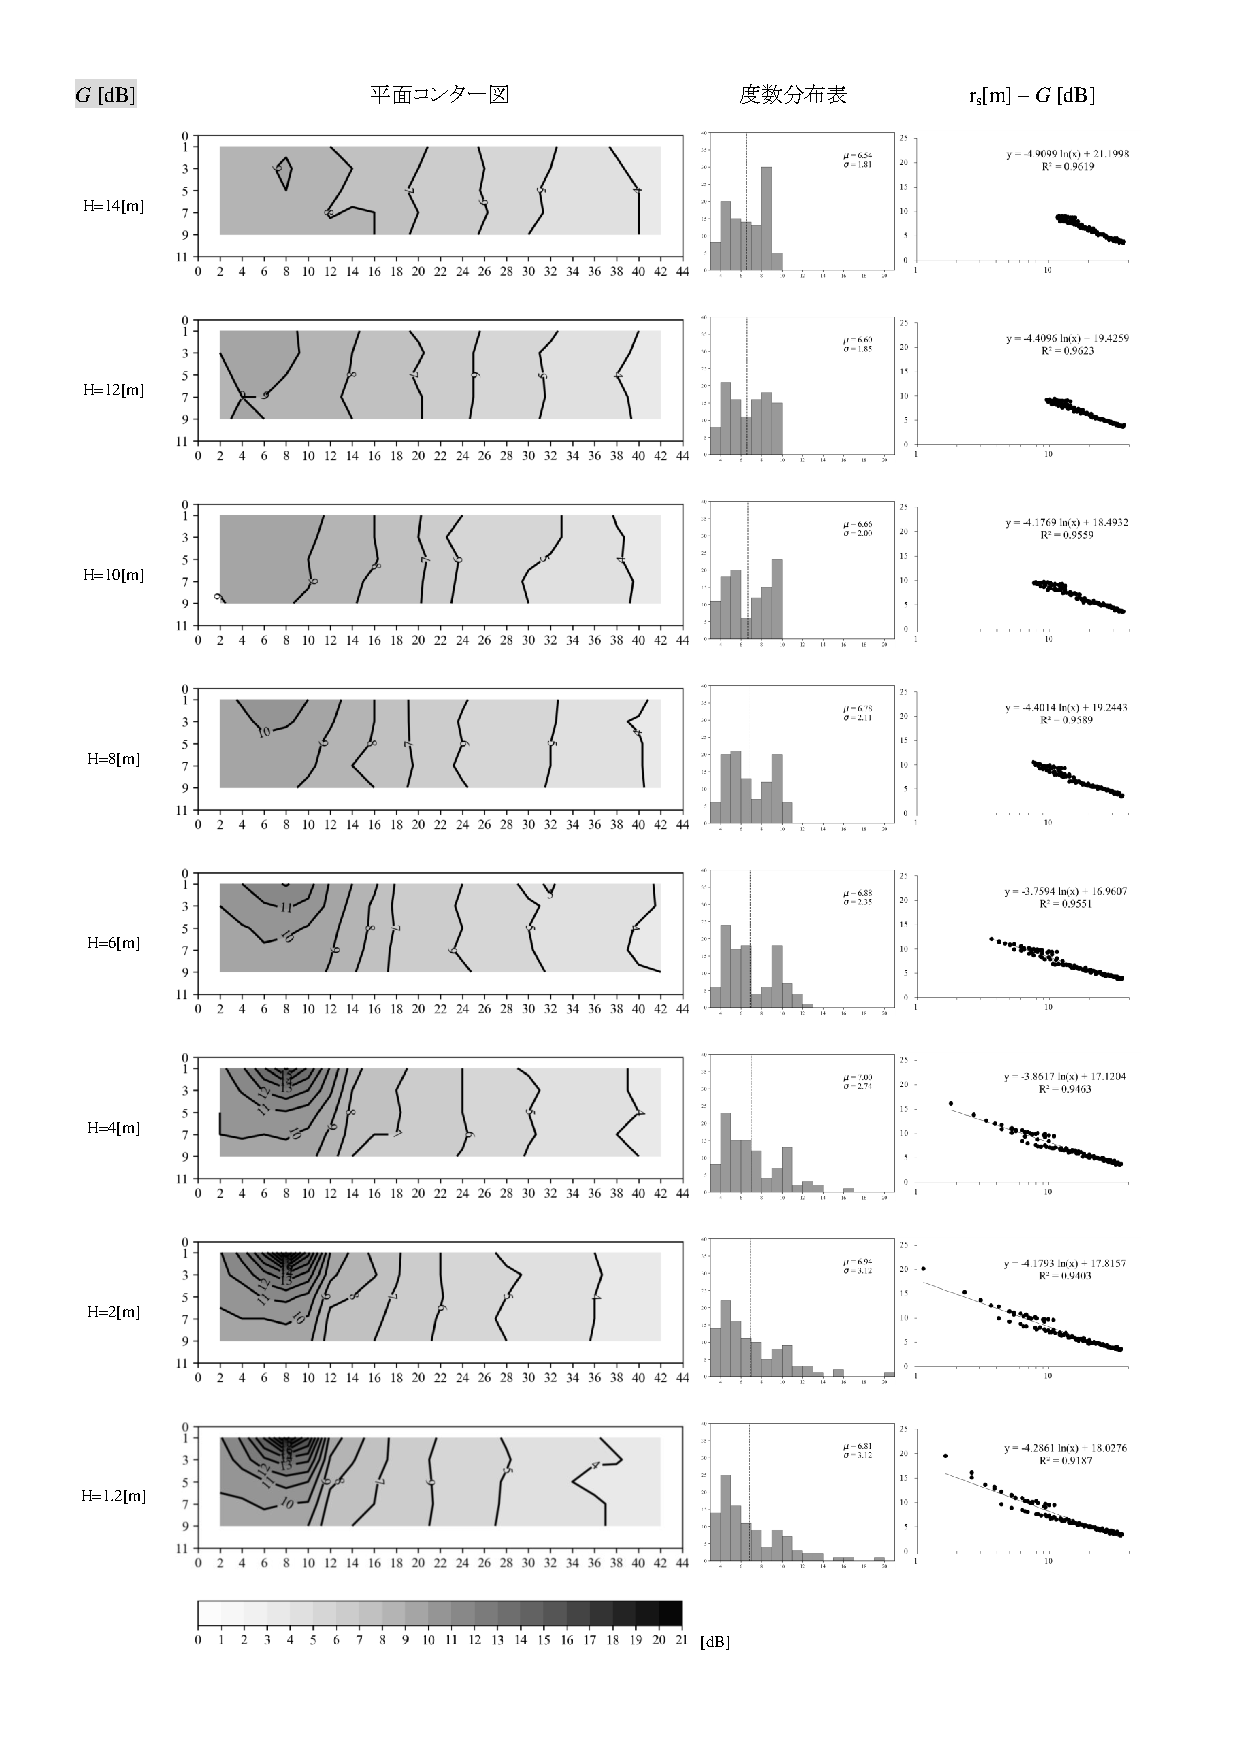
\includegraphics[keepaspectratio,width=1\hsize,angle=0]
                          {04_att/Onkyo_rec3.pdf}
      \end{minipage}
\newpage
      \begin{minipage}{1\hsize}
        \centering
          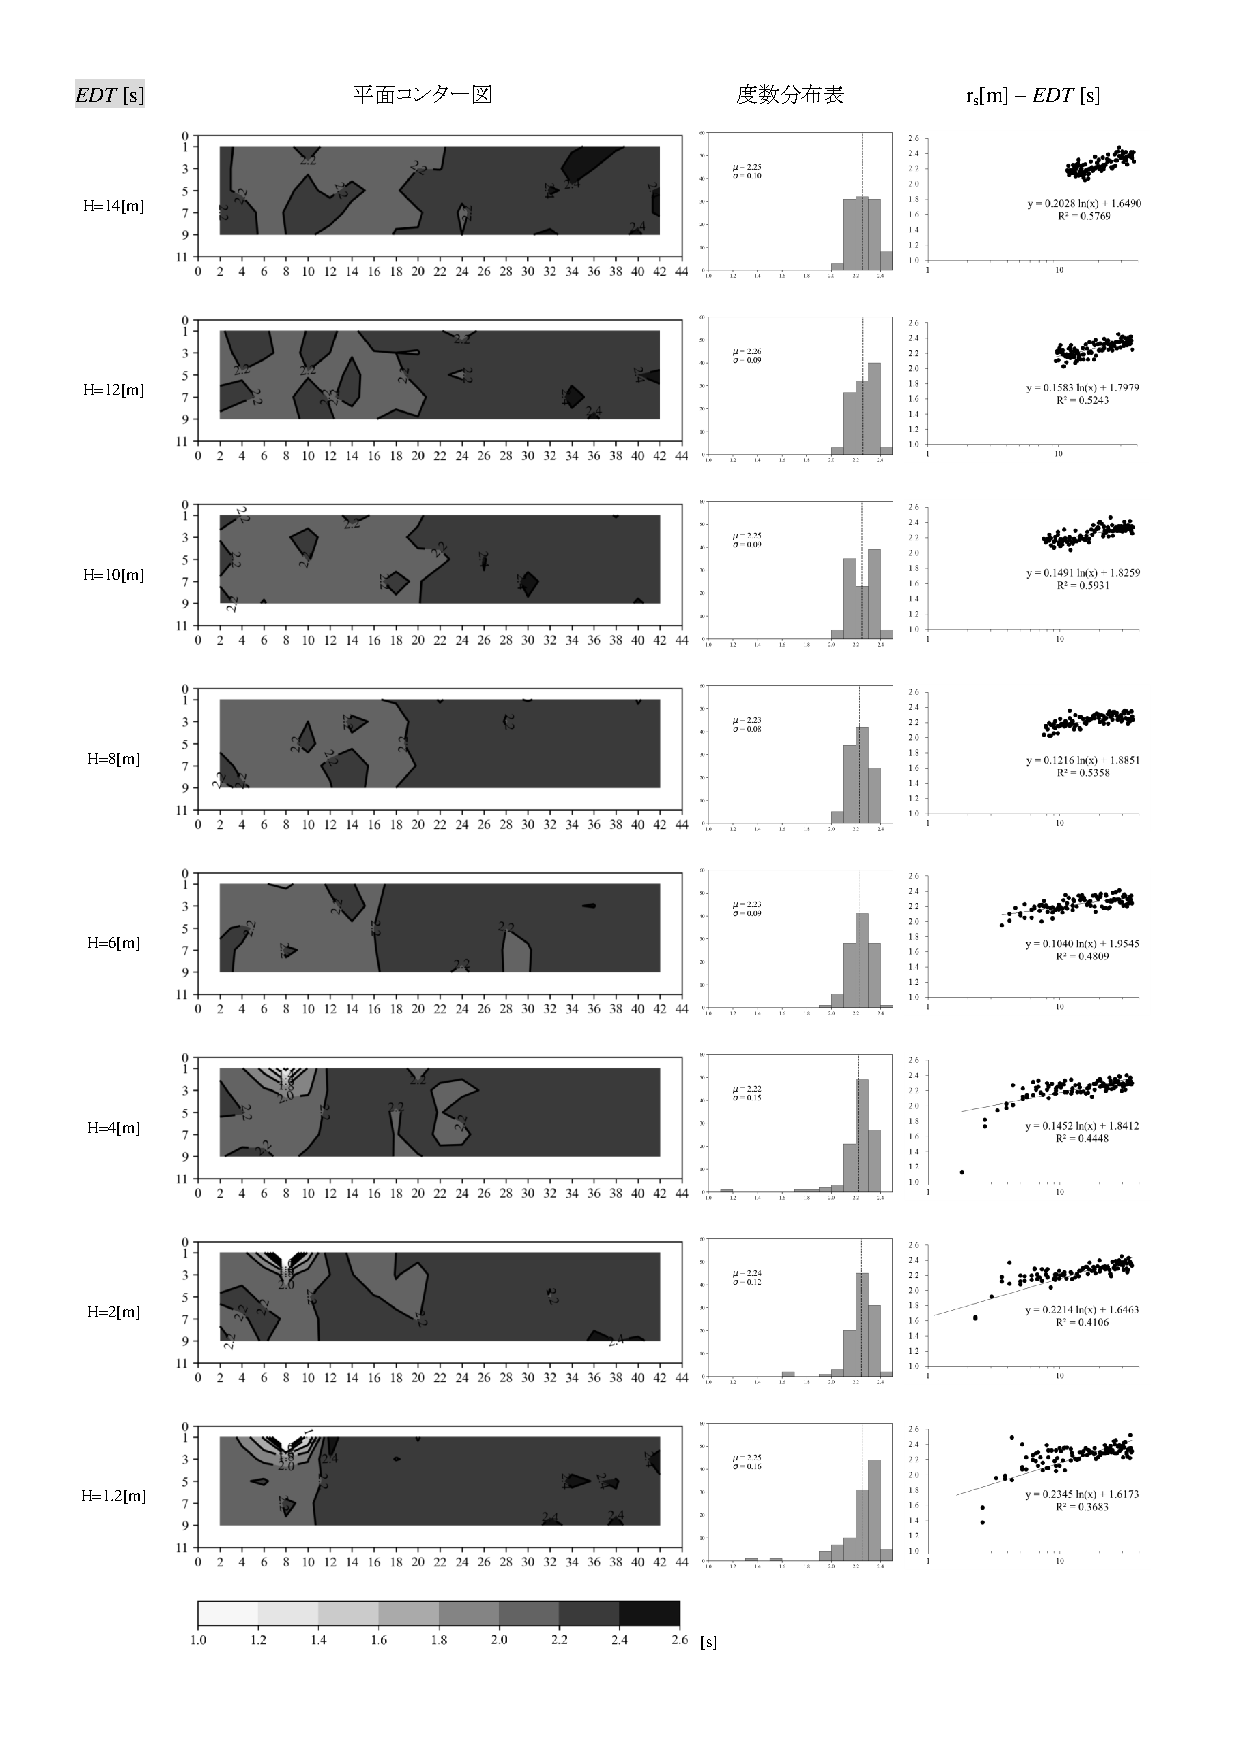
\includegraphics[keepaspectratio,width=1\hsize,angle=0]
                          {04_att/Onkyo_rec4.pdf}
      \end{minipage}
\newpage
      \begin{minipage}{1\hsize}
        \centering
          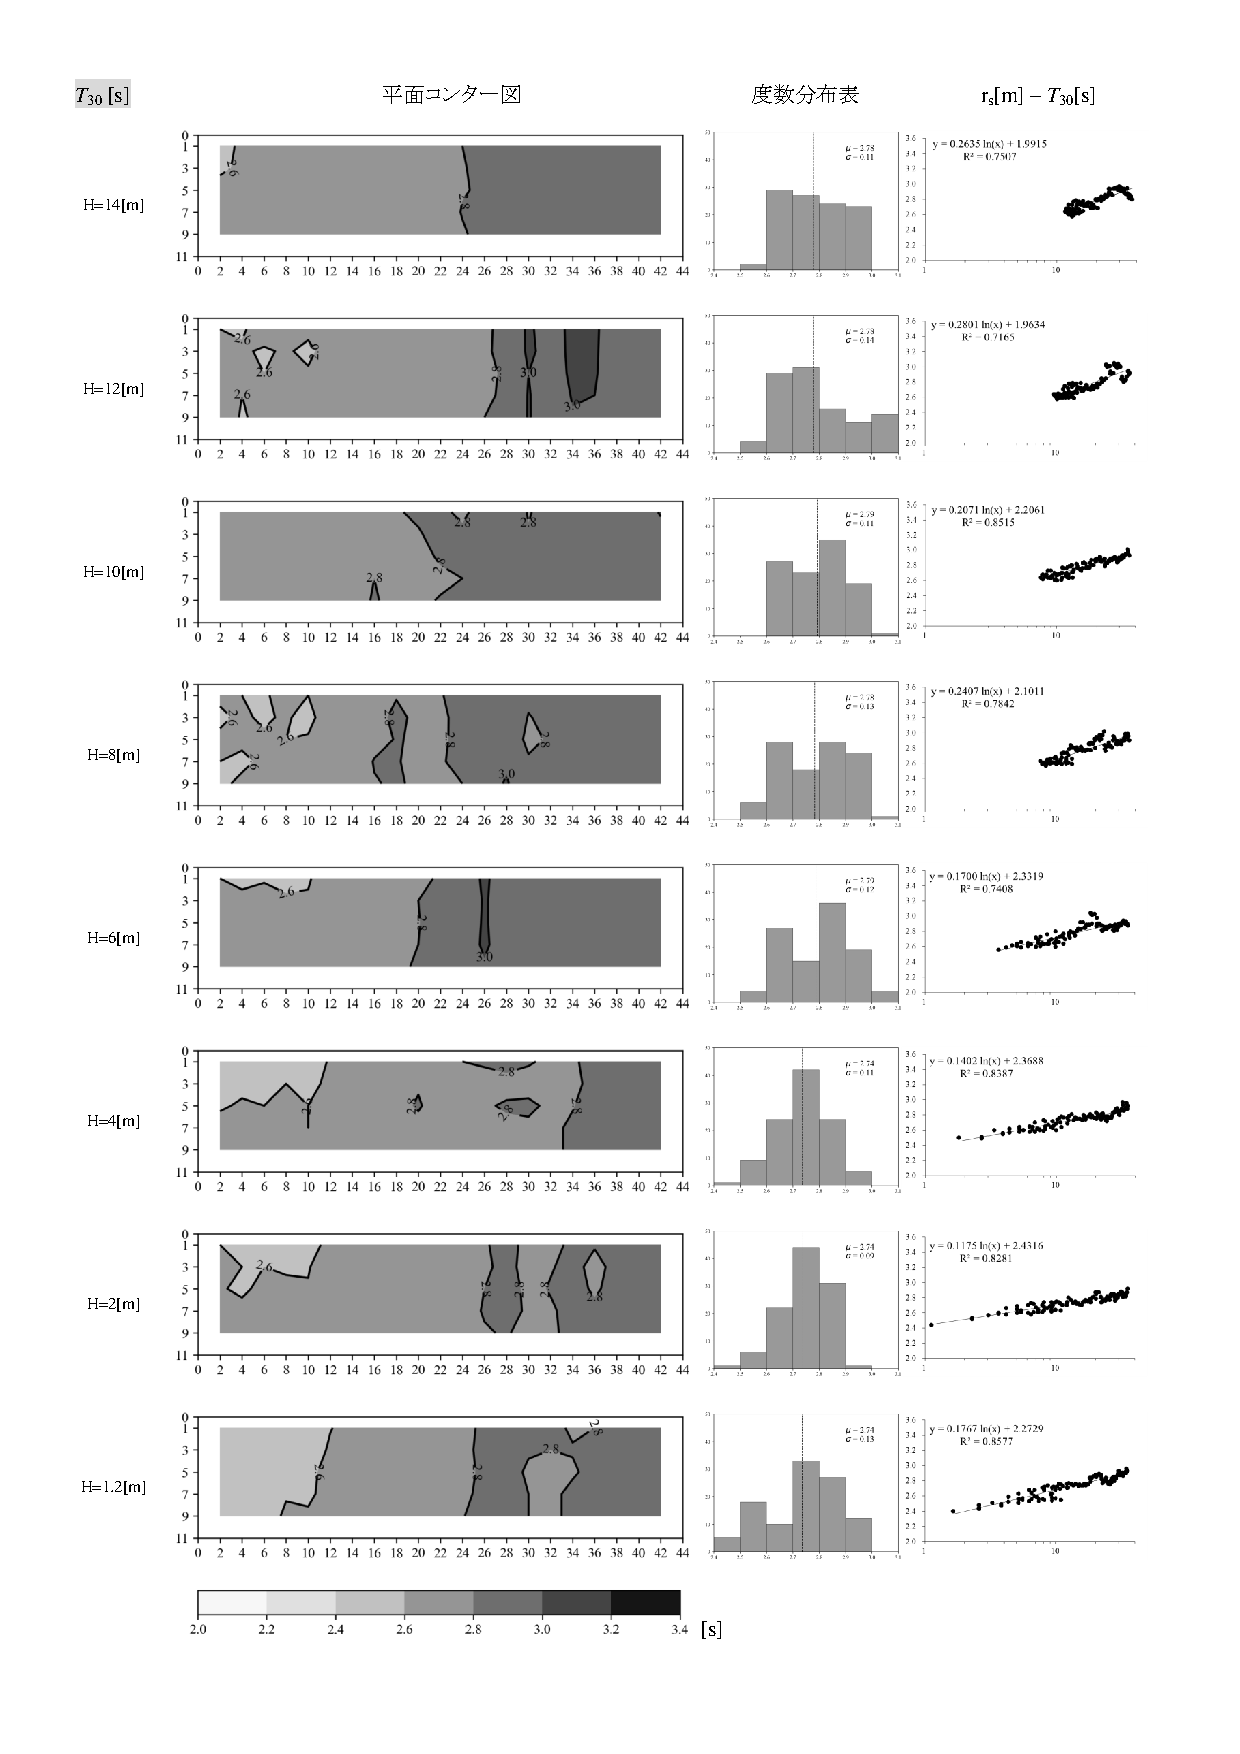
\includegraphics[keepaspectratio,width=1\hsize,angle=0]
                          {04_att/Onkyo_rec5.pdf}
      \end{minipage}
\newpage
      \begin{minipage}{1\hsize}
        \centering
          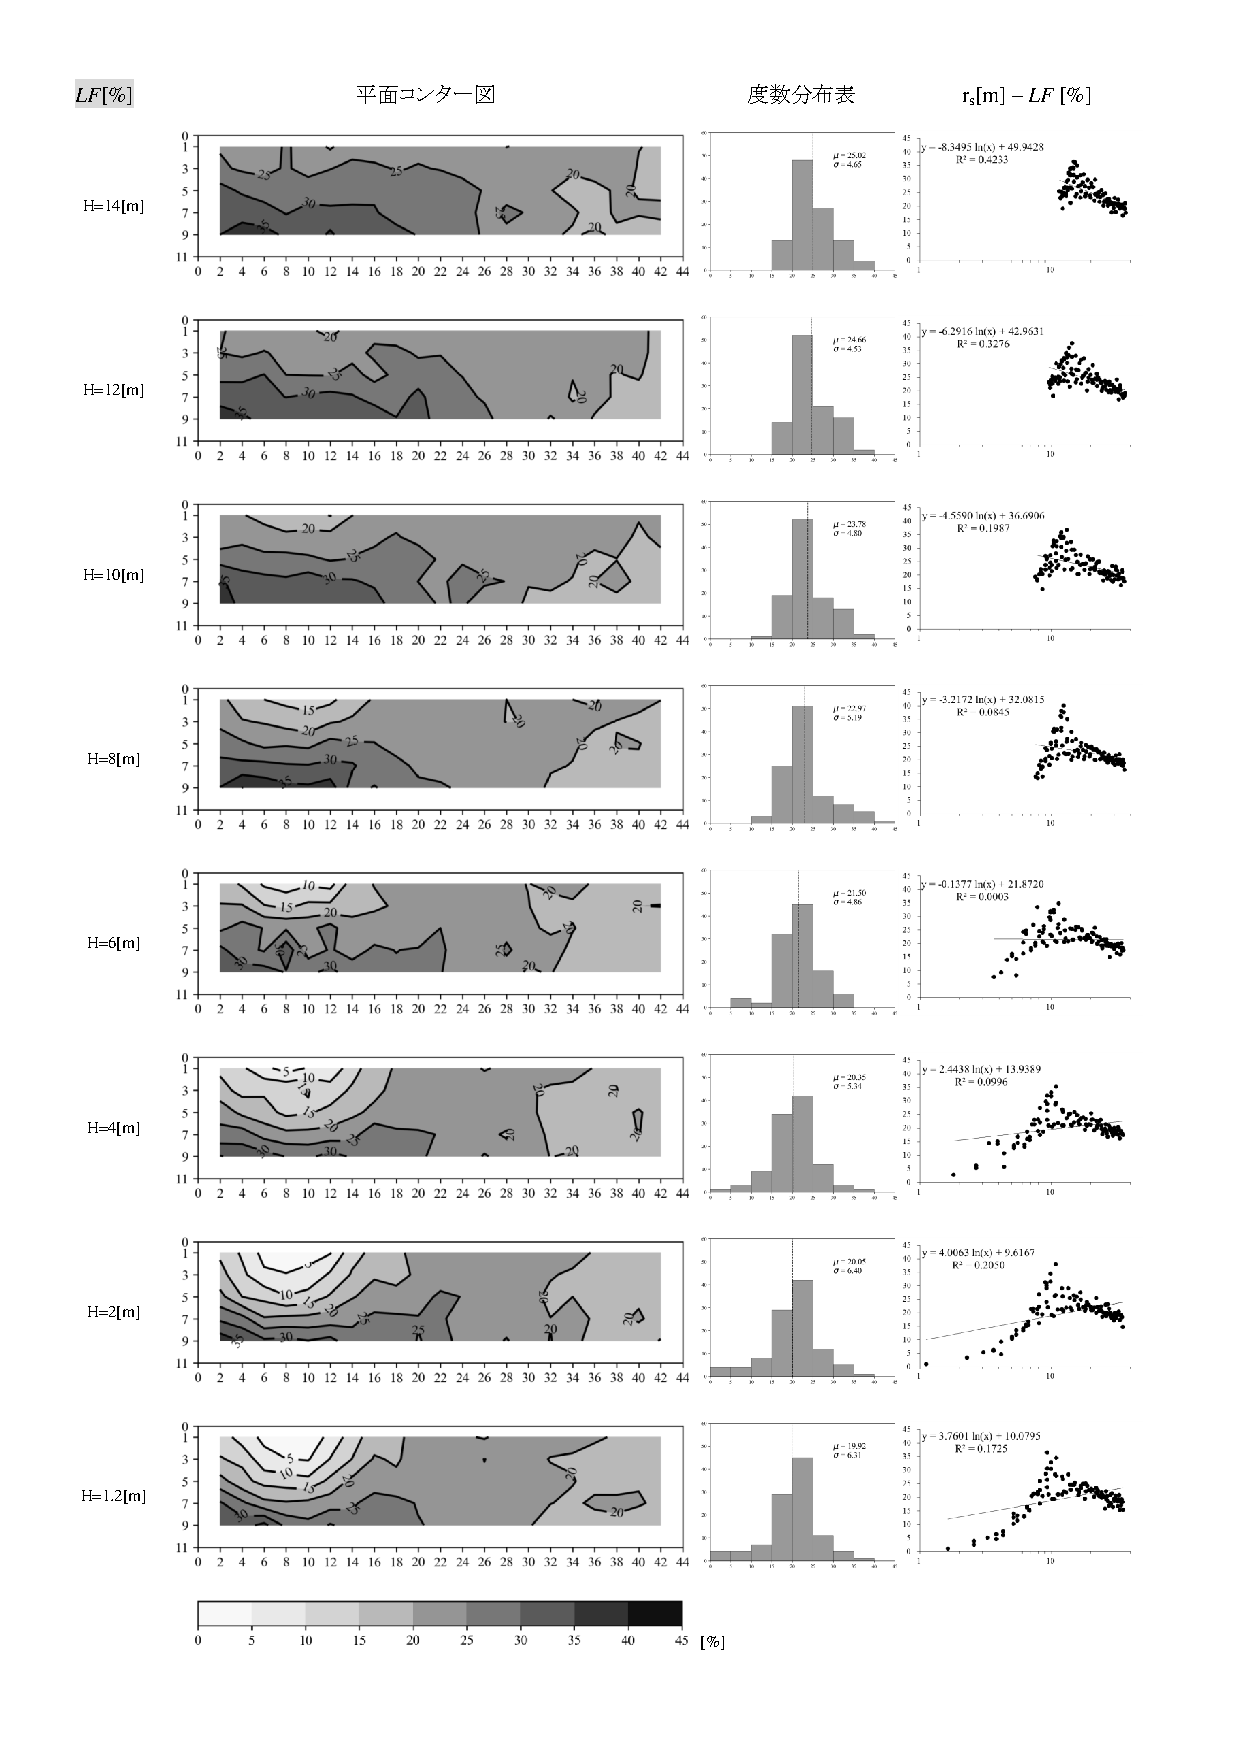
\includegraphics[keepaspectratio,width=1\hsize,angle=0]
                          {04_att/Onkyo_rec6.pdf}
      \end{minipage}      
\newpage
      \begin{minipage}{1\hsize}
        \centering
          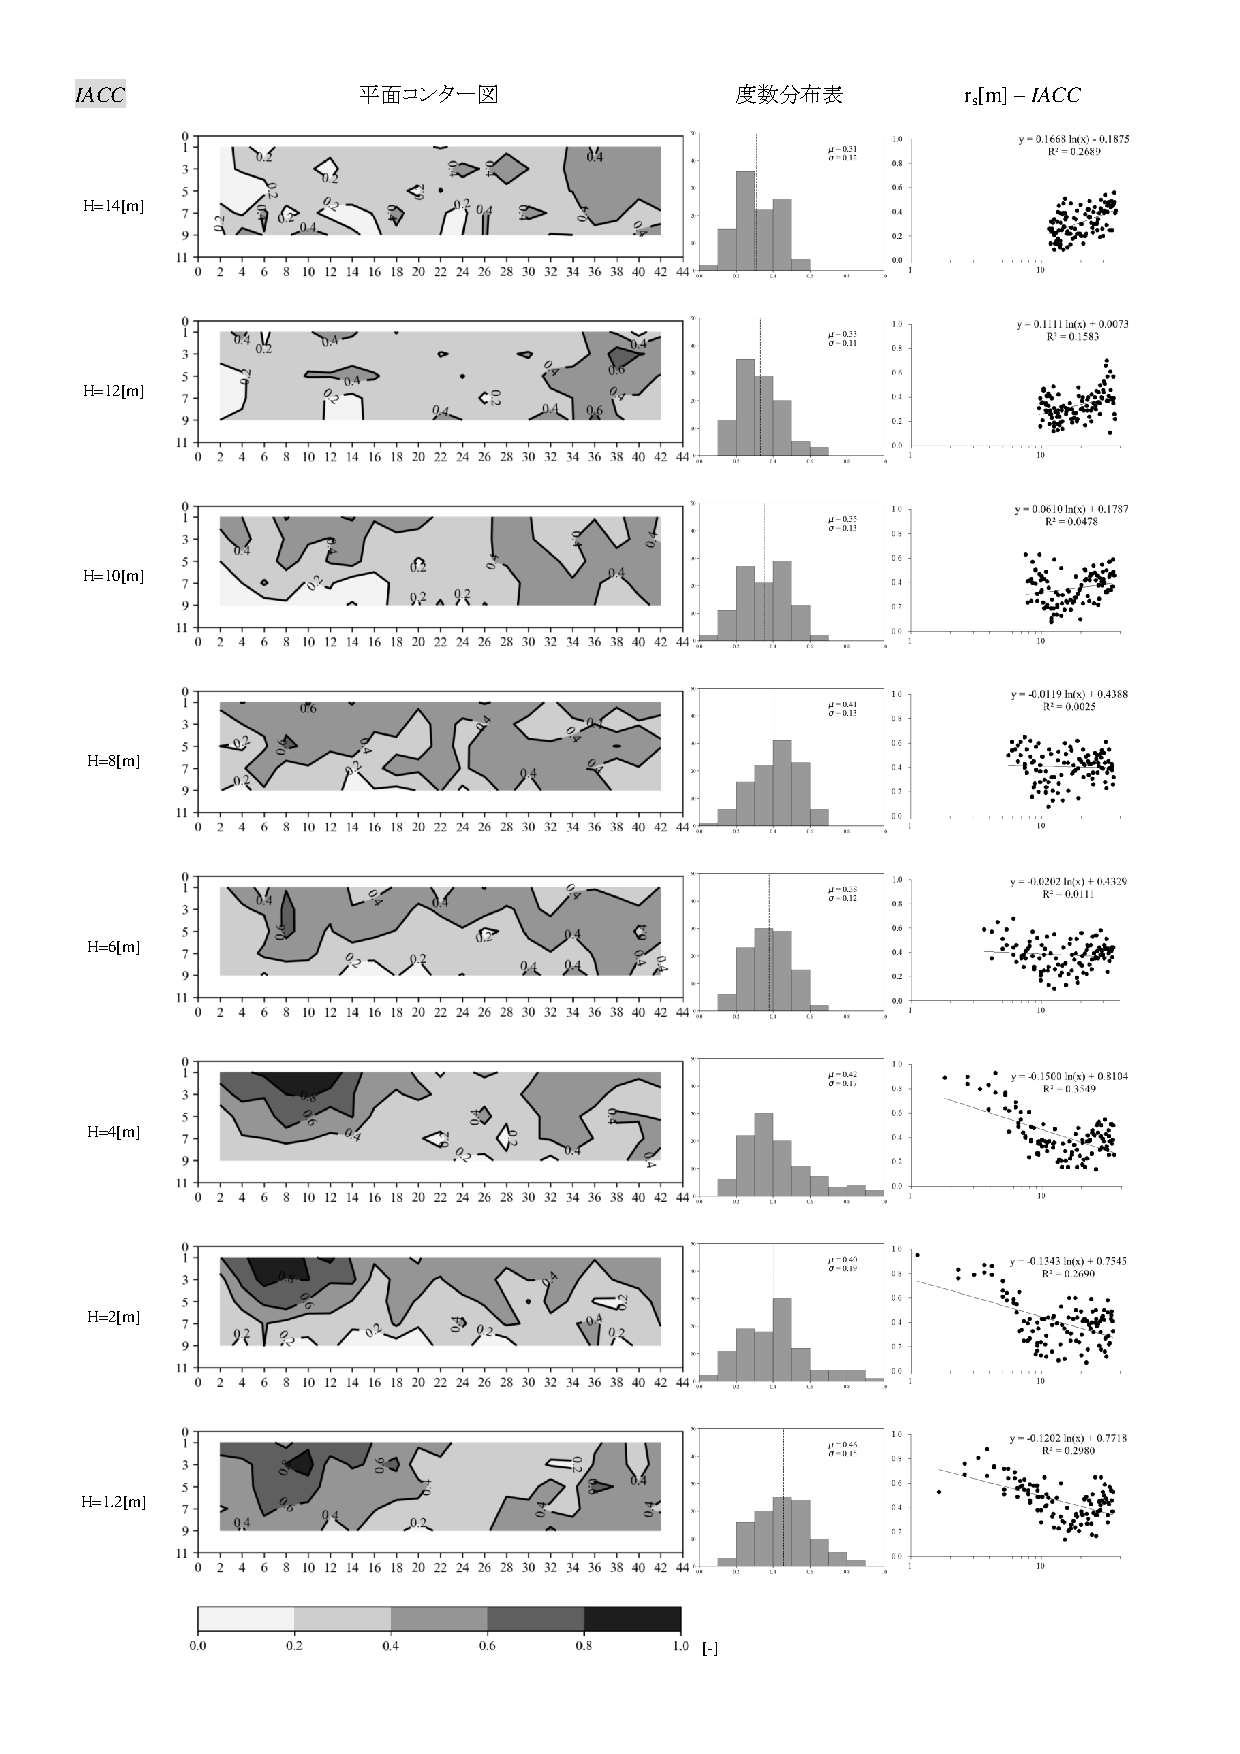
\includegraphics[keepaspectratio,width=1\hsize,angle=0]
                          {04_att/Onkyo_rec7.pdf}
      \end{minipage}      

\section{残響エネルギ特性}
\section{時間エネルギ特性}
\section{音圧レベル特性}
